\subsection{Sprint 3: Testing at scale}
\label{methodoloy:sprint3}
The theme of the third sprint is testing.
Testing is an important part of software development.
It gives the developers certainty over the quality of their program.
We felt like this sprint would be the perfect time to start testing.
It is better to start testing as early as possible.
We started relatively late compared to, for example, the Test Driven Development methodology, where tests are written even before the application logic is written.
However, it has allowed us to quickly iterate on Tsukiji in the early sprints.
At this stage, Tsukiji had reached a level of maturity where logic starts to become significantly more complex.
Tests give us assurance our program works correctly for the test cases we have defined.
There are two forms of testing focused on during this sprint: unit testing and scalibility testing.
Another form of testing that isn't focused on during this sprint is integration testing.
The purpose of integration testing is combine the components of a system and to test whether or not they produce the desired result.
However, at this point tsukiji is still sufficiently small that we believe producing such tests would yield little benefit.

\subsubsection{Unit testing}
Unit testing is the testing of small units of code, ideally the smallest block of code possible.
For our purposes, the smallest block of code is an individual function or class method.
Each unit should be tested in isolation, i.e. each test case is independent of each other.
For unit testing Tsukiji, we use the nosetests library \cite{nosetests}.
nosetests is an extension of the default python unittest library.
With nosetests, it is also possible to measure code coverage.

A large part of what makes testing easy or difficult is expressed in the testability of the code.
How well is the code divided into sufficiently small enough functions, classes and modules?
How large are these components, and how dependant are they upon each other?
Many books, articles, and blog posts have been written on this subject.
An example of such an article is Writing Testable Code\cite{writingtestablecode}, a guide used at Google.
While this guide is written specifically for the Java programming language, its four main points still hold:

\begin{enumerate}
\item Constructor does Real Work
\item Digging into Collaborators
\item Brittle Global State \& Singletons
\item Class Does Too Much
\end{enumerate}

At this point, Tsukiji has two main modules: orderbook.py and trader.py.
The orderbook module consists mainly of functions that concern offers and message creation.

From a unit testing standpoint, the orderbook module is very easy to test.
The functions concerning offers are pure functions, i.e., they have no side-effects.
The functions concerning message creation address a few global variables (e.g. the message counter), but there is a limited amount of these variables and their scope
It could also be said that this module does too much and should be split up.
This is definitely something to keep in mind for the future.

The trader module consists of a relatively large class called Trader.
It implements the DatagramProtocol from the Twisted library.
In essence, very little logic occurs here.
Its main purpose is matching the right message with the right action on the orderbook.
Using the right kind of mocks, this module is also relatively easy to test.

One way of measuring the effectiveness of your tests is by code coverage: how much of your code is run during your tests.
nosetests provides both statement coverage and branch coverage.
Statement coverage is the coverage of each line of code; 100\% statement coverage means that every line of code is run at least once.
Branch coverage is like statement coverage, but takes branches into account.
For example, a boolean condition with one literal has two branches, True or False.
A condition with two literals has four branches.
See figure \ref{coveragefig} for our coverage report.

\begin{figure}
  \centering
  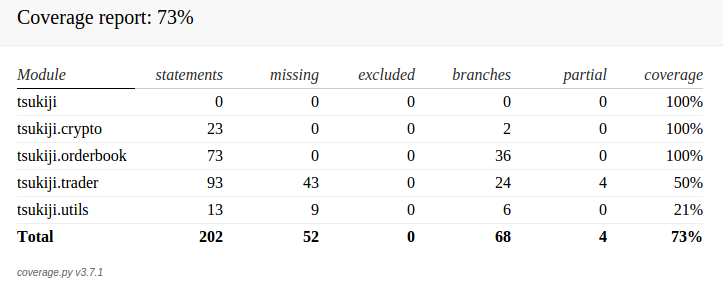
\includegraphics[width=\textwidth]{coverage}
  \caption{A table listing each module's coverage.}
  \label{coveragefig}
\end{figure}


\subsubsection{Scalability testing}
\label{sprint3:scalability}
The other form of testing focused on during this sprint is large scale testing.
The purpose of our large scale test is to test how functional the network remains with a large amount of peers.
Of course, it is not very practical to run our program on hundreds of different devices.
Our solution is to run a simulation locally.
It takes a list of orders and has different peers post those orders in the network.
The tests show that the network could handle thousands of users and that duplicate messages are correctly filtered out.